\documentclass[12pt,a4paper]{article}
\usepackage[utf8]{inputenc}
\usepackage[brazil]{babel}
\usepackage{graphicx}
\usepackage{amssymb, amsfonts, amsmath}
\usepackage{float}
\usepackage{enumerate}
\usepackage[top=2.5cm, bottom=2.5cm, left=1.25cm, right=1.25cm]{geometry}

\begin{document}
\pagestyle{empty}

\begin{center}
  \begin{tabular}{ccc}
    \begin{tabular}{c}
      \includegraphics[scale=0.25]{../../biblioteca/imagem/brasao-de-armas-brasil} \\
    \end{tabular} & 
    \begin{tabular}{c}
      Ministério da Educação \\
      Universidade Federal dos Vales do Jequitinhonha e Mucuri \\
      Faculdade de Ciências Sociais, Aplicadas e Exatas - FACSAE \\
      Departamento de Ciências Exatas - DCEX \\
      Disciplina: Cálculo Numérico \quad Semestre: 2023/2\\
      Prof. Dr. Luiz C. M. de Aquino\\
    \end{tabular} &
    \begin{tabular}{c}
      \includegraphics[scale=0.25]{../../biblioteca/imagem/logo-ufvjm} \\
    \end{tabular}
  \end{tabular}
\end{center}

\begin{center}
  \textbf{Lista II}
\end{center}

\begin{enumerate}
  \item Suponha que o custo para produzir $x$ unidades de certo produto seja aproximadamente 
  dado por $C(x) = \dfrac{1}{2}x^{\frac{2}{3}} + 12x + 1000$. Se esse produto for vendido por
  R\$ 20,00 a unidade, então a partir de qual quantidade não haverá prejuízo? Observação: 
  use o método de Newton na solução.

  \item De uma chapa de alumínio, com dimensão de 30 cm $\times$ 20 cm, serão recortados quatro
  quadrados de lado medindo $x$ cm, como ilustra a figura abaixo. Em seguida, a chapa será dobrada
  de modo a formar uma caixa sem tampa. Determine o valor de $x$ no intervalo [0, 2] para o qual 
  o volume dessa caixa seja 100 cm$^3$. Observação: use o método de Newton na solução com tolerância
  de $10^{-4}$.
  
  \begin{figure}[h]
    \centering
    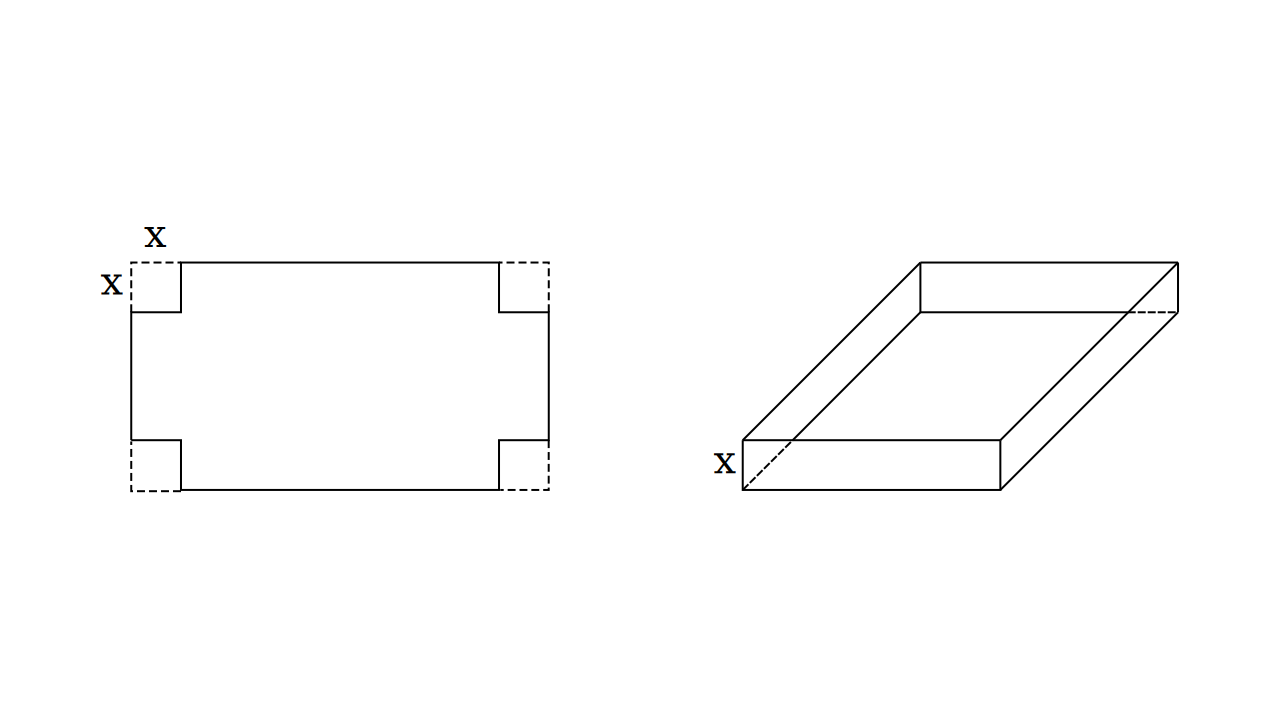
\includegraphics[scale=0.4]{imagem/caixa-retangular.pdf}
  \end{figure}

  \item Use o método de Newton para calcular o valor aproximado de $\sqrt[100]{100}$.
  Observação: use uma tolerância de $10^{-4}$.

  \item Use o método de Newton para determinar o ponto de interseção entre os
  gráficos de $f(x) = \dfrac{1}{x}$ e $g(x) = x^3 + 1$ no primeiro quadrante. 
  Observação: use uma tolerância de $10^{-4}$.
    
\end{enumerate}

\begin{center}
  \textbf{Gabarito}
\end{center}
  \textbf{[1]} A partir de 127 unidades. 
  \textbf{[2]} $x \approx 0,17153705$. 
  \textbf{[3]} $\sqrt[100]{100} \approx 1,04712855$. 
  \textbf{[4]} $x \approx 0,72449196$.
\end{document}